%        File: !comp!expand(``%:p:t'')!comp!
%     Created: !comp!strftime(``%a %b %d %I:00 %p %Y '').substitute(strftime('%Z'), '\<\(\w\)\(\w*\)\>\(\W\|$\)', '\1', 'g')!comp!
% Last Change: !comp!strftime(``%a %b %d %I:00 %p %Y '').substitute(strftime('%Z'), '\<\(\w\)\(\w*\)\>\(\W\|$\)', '\1', 'g')!comp!
\documentclass{anstrans}
%%%%%%%%%%%%%%%%%%%%%%%%%%%%%%%%%%%
\title{Extensions to the Cyclus Ecosystem in Support of Transition Scenario Capability}
\author{Kathryn~D.~Huff$^1$, Massimiliano Fratoni$^1$}

%% uncomment these next five only if using anstrans
\institute{Department of Nuclear Engineering, University of California - Berkeley, Berkeley, CA, 94709}
\email{huff@berkeley.edu}
\usepackage{graphicx}
\usepackage{booktabs} % nice rules for tables
\usepackage{microtype} % if using PDF
\newcommand{\units}[1] {\:\text{#1}}%
\newcommand{\SN}{S$_N$}%{S$_\text{N}$}%{$S_N$}%

\usepackage{multicol}

\date{}
%%%%%%%%%%%%%%%%%%%%%%%%%%%%%%%%%%%
\begin{document}
%%%%%%%%%%%%%%%%%%%%%%%%%%%%%%%%%%%%%%%%%%%%%%%%%%%%%%%%%%%%%%%%%%%%%%%%%%%%%%%%
\section{Introduction}
% Provide a summary of the work conducted:
%      Describe the technical problem clearly
%      support it with a method


Extensions to the Cyclus framework are necessary because the 17 available
institution, region, and facility archetypes packaged with the Cycamore
repository are not quite sufficient to model the specific market-driven
deployment and fuel fabrication specifications in the transition scenario
definition of interest. This is a canonical example of the need for extension
capability in Cyclus. That is, each scenario specification of interest in fuel
cycle analysis is usually sufficiently pathological that modifications must
almost always be made in any simulation framework. The modularity built into
the Cyclus framework allows extension without modification of the core logic.  

In this work, support archetype models have been developed to extend the
capabilities of the Cyclus ecosystem. Those model implementations are described
as are the capabilities that they contribute. 
 

%%%%%%%%%%%%%%%%%%%%%%%%%%%%%%%%%%%%%%%%%%%%%%%%%%%%%%%%%%%%%%%%%%%%%%%%%%%%%%%%
\section{Simulation Description}
\subsection{Scenario Definition}

The simulation starts in January 2014 and lasts until transition to 100\% SFRs 
is complete. The nuclear installed capacity is constant (100GWe).


\subsubsection{Commodities}

%\begin{multicols}{1}
\begin{table}[h!]
\centering
\begin{tabular}{|l|l|l|}
\hline
Commodity  &     Offered By  &    Requested By \\
\hline
Natural  U & Mine & Enrichment \\ 
LEU & Enrichment & LWRFuelFab \\ 
Depleted  U & Enrichment & SFRFuelFab \\ 
fresh  LWR  fuel & LWRFuelFab & LWR \\ 
fresh  SFR  fuel & SFRFuelFab & SFR \\ 
LWR  UNF & LWR & LWRWetStorage \\ 
SFR  UNF & SFR & SFRWetStorage \\ 
cool LWR  UNF & LWRWetStorage & LWRSeparations \\ 
cool SFR  UNF & SFRWetStorage & SFRSeparations \\ 
Reprocessed  LWR  U & LWRSeparations & SFRFuelFab \\ 
Reprocessed  LWR  TRU & LWRSeparations & SFRFuelFab \\ 
Reprocessed  SFR  U & SFRSeparations & SFRFuelFab \\ 
Reprocessed  SFR  TRU & SFRSeparations & SFRFuelFab \\ 
\hline
\end{tabular}
\caption{Commodity movement in the transition simulation}
\label{tab:commods}
\end{table}
%\end{multicols}

Note that the exact compositions of U and TRU were not given. These will be
approximated by representative isotopes in the Cyclus definition.


\subsubsection{Facility Implementations}

\onecolumn
\begin{table}
\centering
\begin{tabular}{|l|l|r|}
\hline
\textbf{Facility Type} &\textbf{Model} & \textbf{Parameters}\\
\hline
Mine & SourceFacility & Capacity = Unlimited\\
Enrichment & EnrichmentFacility & Natural U enrichment = 0.711 wt\% \\
& & Depleted U enrichment =  0.25 wt\% \\
& & ''Enrichment Time'' for LWR fuel = 1 year\\
LWRFuelFab & StreamBlender & Fabrication time = 1 year\\
& & Fissionable material source = 4.3\% LEU\\
SFRFuelFab & StreamBlender  & Fabrication time = 1 year\\
& & fissile material = rep sfr tru, rep lwr tru \\
& & fertile material = rep sfr u, rep lwr u, dep u, nat u \\
LWR & BatchReactor & 1000 MWe per reactor \\
& & 0.90 Capacity Factor \\
& & 3 batches per core \\ 
& & Deployment : initial 2014 deployment only (100 LWRs) \\
& & Decommissioning : decommission 1 LWR per 3 SFRs built \\
& & Burnup = 50 MWd/kgIHM \\
& & Cycle length = 1.5 calendar years \\
& & Licensing time = 2 years \\
& & Construction time = 4 years \\
& & goal recipe \\
SFR & BatchReactor & 333.3 MWe per reactor (1000/3) \\
& & 0.90 Capacity Factor \\
& & Deployment : deploy 3 when 83515 tons LWR UNF available \\ 
& & Decomissioning (after 60 years) \\
& & 3.3 batches per core? \\ 
& & Burnup = 73 MWd/kgIHM \\
& & Cycle length = 1.3 calendar years \\
& & Licensing time = 2 years \\
& & Construction time = 4 years \\
LWRWetStorage & CommodConverter & process time = 4 years\\
SFRWetStorage & CommodConverter & process time = 1 year \\
LWRWetSeparations & SeparationsMatrix & Start Date : when needed\\
& & Unlimited Capacity\\
& & No reprocessing losses\\
SFRWetSeparations & SeparationsMatrix & Start Date : when needed\\
& & Unlimited Capacity\\
& & No reprocessing losses\\
\hline
\end{tabular}
\caption{Facilities and their Implementations in the simulation.}
\label{tab:facimpl}
\end{table}
\twocolumn


\subsubsection{Desired Outputs}
The desired outputs of this simulation include deployment metrics such as the 
year during which the transition becomes complete and capacity profiles over 
time. These profiles should demonstrate that there were no potential generating 
shortages. Additionally, material metrics such as separated surplus PU or TRU 
profiles, LWR used fuel reprocessing rate (t/yr), SFR used fuel reprocessing 
rate (t/yr),  LWR used fuel mass in storage (t), and SFR used fuel mass in 
storage (t).

\subsection{Existing Capabilities}

A number of exsiting capabilities were used to acheive this simulation. One is 
the GrowthRegion, which can maintain a power profile according to a demand 
curve. Another is the BatchReactor, which generically represents multi-batch reactor 
models with fresh and spent fuel material compositions defined by the user. The 
Source Facility and Sink Facility produce and consume material, respectively. 
Accordingly, they represent the Mine and HLW Repository in this simulation.  

\input{capabilitygap}

%%%%%%%%%%%%%%%%%%%%%%%%%%%%%%%%%%%%%%%%%%%%%%%%%%%%%%%%%%%%%%%%%%%%%%%%%%%%%%%%
\section{Module Extensions}

\subsection{Commodity Converter Facility}

One versatile facility model contributed by this work is a simple 
representation of timed storage. After recieving material, this facility 
waits for a user-defined time period. Once that time period has passed, the 
material object is offered up as a new commodity type. 

In the case of a storage facility, for example, this model requests a commodity 
such as spent fuel, then waits for a cooling period before offering the same 
material as cooled spent fuel.

\begin{table}[h!]
\centering
\begin{tabular}{|l|r|r|r|}
\hline
\textbf{Parameter} & \textbf{Units} & \textbf{Default} & \textbf{Range}\\
\hline
Input Commodity& string & ``'' & any string\\
Output Commodity& string & ``'' & any string\\
Delay Time & months & $0$ & $0-\infty$\\
Storage Capacity & kg & \infty &$0-\infty$ \\
\hline
\end{tabular}
\caption{Input parameters for the Commodity Converter Facility Model}
\label{tab:commodconverter}
\end{table}


% --------------------------------------------------------------
\begin{frame}[fragile]
  \frametitle{Stream Blender} 
The process specified for SFR fuel fabrication from separated materials streams
can most concisely be described as blending into a recipe.
\begin{figure}[htbp!]
\begin{center}
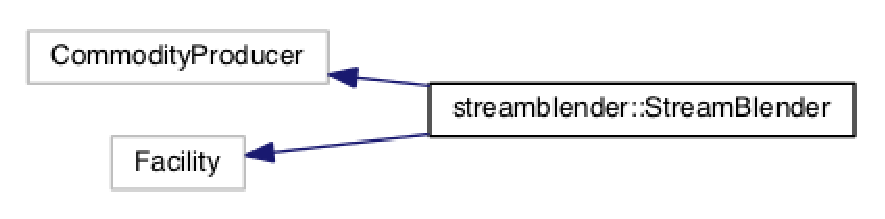
\includegraphics[width=0.8\textwidth]{sb_inherit}
\end{center}
\caption{Utilizes interfaces defined in Cyclus.}
\label{fig:sb_inherit}
\end{figure}
\end{frame}
% --------------------------------------------------------------
\begin{frame}[fragile]
  \frametitle{Stream Blender}
This new StreamBlender Facility Agent 
(\url{https://katyhuff.github.io/StreamBlender}) 
\cite{huff_market_2014} handles the combination of various commodity streams in 
appropriate proportions to achieve a goal recipe.  

\begin{itemize}
\item incoming commodities
\item incoming recipes
\item outgoing commodity
\item goal recipe
\item driving isotopes and sources
\item waste commodity (default = ''waste``)
\item process time (default = 0)
\end{itemize}
\end{frame}
% --------------------------------------------------------------
\begin{frame}[fragile]
\footnotesize{
\begin{lstlisting}
  <facility>
    <name>SFRFuelFab</name>
    <lifetime>1200</lifetime>
    <config>
      <StreamBlender>
        <in_commods>
          <val>rep_sfr_tru</val>
          <val>rep_lwr_tru</val>
          <val>rep_sfr_u</val>
          <val>dep_u</val>
          <val>nat_u</val>
        </in_commods>
        <out_commod>fresh_sfr_fuel</out_commod>
        <out_recipe>fresh_sfr_fuel_recipe</out_recipe>
        <in_recipes>
          <val>rep_sfr_tru_recipe</val>
          <val>rep_lwr_tru_recipe</val>
          <val>rep_sfr_u_recipe</val>
          <val>dep_u_recipe</val>
          <val>nat_u_recipe</val>
        </in_recipes>
\end{lstlisting}
}
\end{frame}
% --------------------------------------------------------------
\begin{frame}[fragile]
\footnotesize{
\begin{lstlisting}
        <isos>
          <val>94240</val>
          <val>94240</val>
          <val>92235</val>
          <val>92235</val>
          <val>92235</val>
          <val>94239</val>
          <val>95241</val>
        </isos>
        <sources>
          <val>rep_sfr_tru</val>
          <val>rep_lwr_tru</val>
          <val>rep_sfr_u</val>
          <val>dep_u</val>
          <val>nat_u</val>
          <val>rep_lwr_tru</val>
          <val>rep_lwr_tru</val>
        </sources>
        <process_time>12</process_time>
      </StreamBlender>
    </config>
  </facility>
\end{lstlisting}
}
\end{frame}

\subsection{Matrix-Based Separation Facility Model}

By describing the separations process as a simple matrix of efficiencies, a 
simple 1:N material stream transformation is conducted. The specific process 
chemistry for the separation at hand is treated as elemental, as representative 
of a non-laser separations process. The matrix of separation efficiencies has a 
default value: the identity matrix. In this context, the identity matrix 
represents complete and perfect elemental separation without losses. 

\begin{align}
  \left[
    \begin{array}{c c c c c c c}
      \eta_{11} & . & . & . & . & . & \eta_{1M} \\
      \eta_{21} & . & . & . & . & . & \eta_{2M} \\
      . & . & . & . & . & . & . \\
      . & . & . & . & . & . & . \\
      . & . & . & . & . & . & . \\
      \eta_{N1} & .  & . & . & . & . & \eta_{NM} \\
    \end{array}
    \right]
  \left[
    \begin{array}{c}
      I_1\\
      I_2\\
      . \\
      . \\
      . \\
      I_N\\
    \end{array}
    \right]
    =
    \left[
      \begin{array}{ c }
        E_1\\
        E_2\\
        .\\
        .\\
        .\\
        E_M\\
      \end{array}
      \right]
\label{defaultsep}
\end{align}

Thus, for realistic separations, the user is expected to produce an efficiency 
matrix representing the separations technology of interest to them. 
By requesting the feedstock from the 
appropriate markets, the facility acquires an unseparated feedstock stream. 
Based on the input parameters  in Table \ref{tab:sepmatrix}, the separations 
process proceeds within the timesteps and other constraints of the simulation. 


\begin{table}[h!]
\centering
\begin{tabular}{|l|r|r|r|}
\hline
\textbf{Parameter} & \textbf{Units} & \textbf{Default} & \textbf{Range}\\ 
\hline
& & & \\
\hline
\end{tabular}
\caption{Input parameters for the Matrix-Based Separation Facility Model}
\label{tab:sepmatrix}
\end{table}

Thereafter, separated streams as well as a stream of losses are offered the 
appropriate markets for consumption by other facilities. In the transition 
scenario at hand, the StreamBlender fuel fabridation facility purchases the 
streams it desires in order to produce SFR fuel. 


\label{sec:decomminst}
\subsection{Deommissioning Institution}
The new Institution Agent was based on an already existing institution
model, but required a market-based look-ahead deployment capability to
faithfully model this scenario. 

That is, by relying on inheritance from a mixin class already available within 
the \Cyclus toolkit, an institution can deploy and decommission facilities 
based on any decision criteria. By also relying on the dynamic resource 
exchange interface, it is possible to base that decision criteria on the 
availability of resources being offered by other facility agents in the 
simulation. 

In this case, a specific quantity of separated transuranic material must exist 
before an LWR can be decommissioned (to be replaced with three SFRs). That 
decision criteria, combined with the capability of decommissioning facilities, 
gives the Decommisioning Institution. 




%%%%%%%%%%%%%%%%%%%%%%%%%%%%%%%%%%%%%%%%%%%%%%%%%%%%%%%%%%%%%%%%%%%%%%%%%%%%%%%%
\section{Results and Analysis}
% Provide your results:
%       clearly

To extend the capabilities of the \Cyclus ecosystem to include market-driven 
building and decommissioning, physics agnostic separations, simple storage, and 
source-preferential fuel fabrication, the following Agents were developed:

\begin{itemize}
\item SeparationsMatrix Facility, physics agnostic separations
\item CommodConverter Facility, timed-release storage
\item StreamBlender Facility, source-preferential fuel fabrication 
\item MktDrivenInst, a market-driven institution.
\end{itemize}



\section{Acknowledgements}

This work was conducted <LLNL text>.

Additionally, this material is based upon work supported by the Department of 
Energy National Nuclear Security Administration under Award Number(s) 
DE-NA0000979. % Katy's appointment is NSSC, must acknowledge for everything

<disclaimer text>.



%%%%%%%%%%%%%%%%%%%%%%%%%%%%%%%%%%%%%%%%%%%%%%%%%%%%%%%%%%%%%%%%%%%%%%%%%%%%%%%%
\bibliographystyle{ans}
\bibliography{bibliography}
\end{document}


